\begin{frame}
    \frametitle{What are we going to be talking about?}
    \pause
    \centering
    \LARGE
    Digital circuits!

    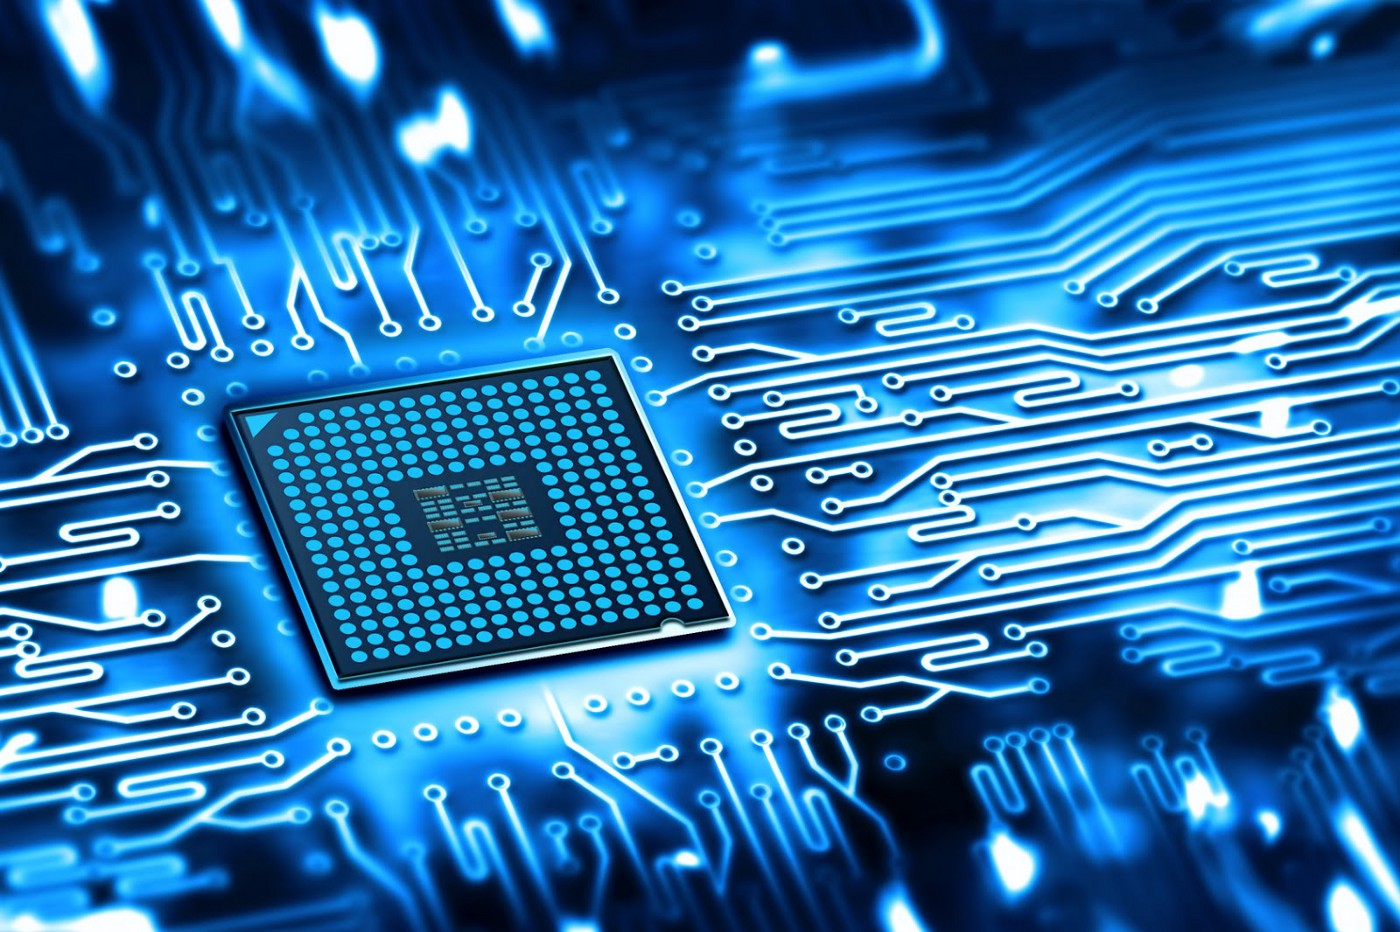
\includegraphics[width=0.6\textwidth]{imgs/circuit}
\end{frame}
\begin{frame}
    \frametitle{What are we going to be talking about?}
    \centering
    \LARGE
    Digital circuits!

    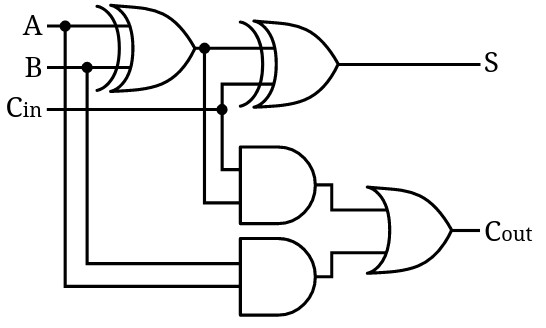
\includegraphics[width=0.6\textwidth]{imgs/adder}
\end{frame}
\begin{frame}
    \frametitle{What are we going to be talking about?}

    \pause

    \centering
    \LARGE
    We want a \alert{compositional} theory of digital circuits.

    \vspace{0.5em}

    \normalsize

    \pause
    F g

    \vspace{0.5em}
    Composites

    \pause
    \vspace{0.5em}

\end{frame}
\begin{frame}
    \frametitle{But why do we want that?}
    \centering
    \LARGE
    We want to reason \alert{equationally} about circuits.

    \normalsize
    Example rewrite of circuits (definition of rewrite will do)

\end{frame}
\begin{frame}
    \frametitle{Why all the pictures?}
    \centering
    \LARGE
    String diagrams are \alert{good}.

    \normalsize
    (but these are a little different to the ones Dan and Jamie are using)

    put some pictures on this slide too

\end{frame}